\documentclass[conference]{IEEEtran}
\IEEEoverridecommandlockouts
% The preceding line is only needed to identify funding in the first footnote. If that is unneeded, please comment it out.
%Template version as of 6/27/2024

\usepackage{cite}
\usepackage{amsmath,amssymb,amsfonts}
\usepackage{algorithmic}
\usepackage{graphicx}
\usepackage{textcomp}
\usepackage{xcolor}
\usepackage{url}
\usepackage{multirow}
\usepackage{mathrsfs}
\usepackage{booktabs}
% \usepackage{xeCJK} % 加载xeCJK宏包
% \setCJKmainfont{SimSun} % 设置中文主字体为宋体

\def\BibTeX{{\rm B\kern-.05em{\sc i\kern-.025em b}\kern-.08em
    T\kern-.1667em\lower.7ex\hbox{E}\kern-.125emX}}
\begin{document}

\title{Legal Ethics Assistant: An Integrated Framework for Legal-Ethical Risk Analysis\\
% Article-enhanced Pre-trained Language Model for LegalCase Retrieval
% {\footnotesize \textsuperscript{*}Note: Sub-titles are not captured for https://ieeexplore.ieee.org  and should not be used}
% \thanks{Identify applicable funding agency here. If none, delete this.}
}

\author{\IEEEauthorblockN{1\textsuperscript{st} Yanqing An}
\IEEEauthorblockA{\textit{School of Artificial Intelligence and Data Science} \\
\textit{University of Science and Technology of China}\\
Hefei, China \\
anyq@mail.ustc.edu.cn}}
% \and
% \IEEEauthorblockN{2\textsuperscript{nd} Given Name Surname}
% \IEEEauthorblockA{\textit{dept. name of organization (of Aff.)} \\
% \textit{name of organization (of Aff.)}\\
% City, Country \\
% email address or ORCID}
% \and
% \IEEEauthorblockN{3\textsuperscript{rd} Given Name Surname}
% \IEEEauthorblockA{\textit{dept. name of organization (of Aff.)} \\
% \textit{name of organization (of Aff.)}\\
% City, Country \\
% email address or ORCID}
% \and
% \IEEEauthorblockN{4\textsuperscript{th} Given Name Surname}
% \IEEEauthorblockA{\textit{dept. name of organization (of Aff.)} \\
% \textit{name of organization (of Aff.)}\\
% City, Country \\
% email address or ORCID}
% \and
% \IEEEauthorblockN{5\textsuperscript{th} Given Name Surname}
% \IEEEauthorblockA{\textit{dept. name of organization (of Aff.)} \\
% \textit{name of organization (of Aff.)}\\
% City, Country \\
% email address or ORCID}
% \and
% \IEEEauthorblockN{6\textsuperscript{th} Given Name Surname}
% \IEEEauthorblockA{\textit{dept. name of organization (of Aff.)} \\
% \textit{name of organization (of Aff.)}\\
% City, Country \\
% email address or ORCID}
% }

\maketitle

\begin{abstract}
    With the growth of large language models and artificial intelligence, AI-based tools are increasingly being adopted. These technological advances bring convenience but also raise ethical concerns. For example, ordinary people may become embroiled in disputes or face unforeseen entrepreneurial risks. Non-professionals can obtain information about the potential consequences of an event from commercially available legal tools, while lawyers and other professionals can assess cases by searching case databases and generating similar-case reports. However, the results obtained in this way are often incomplete and drawn from multiple, fragmented sources. To provide a faster and more information-rich understanding of the potential consequences of an event, we propose the Legal Ethics Assistant. Specifically, we integrate lawyer competence assessment, legal judgment prediction, similar-case retrieval, and large language models to provide users with information relevant to the facts of a case, thereby assisting them in considering legal and ethical risks at the early stages of an entrepreneurial idea or a legal case.
% 类案检索旨在根据案件事实检索相似的案件，是法律智能中具有意义的任务。近年来，预训练模型被用于类案检索任务中，但针对案件的组成元素仍未被充分利用。与搜索引擎相比，法律文书的检索更加专业，法律文本更加结构化且文本长度更长。现有的类案检索方法利用了法律文本的半结构化属性，将法律文书分为了facts，holdings，judgment等部分。为了充分发挥类案检索模型的能力，我们将法条加入了预训练模型辅助训练。在公开可用的法律基准数据集上进行的大量实验表明，我们的方法在法律案件检索任务上具有有效性。
\end{abstract}

\begin{IEEEkeywords}
    Legal intelligence, ethics, service
% Legal intelligence, retrieval, article.
\end{IEEEkeywords}

\section{Introduction}

% 背景
% https://www.youtube.com/watch?v=bZNtCQCA6VY
In recent years, with the rise of digital humans~\cite{zhang2025intelligent} and agentic reinforcement learning technologies, artificial intelligence has begun to be widely applied. While these advances bring convenience, they also raise ethical concerns. For example, ordinary people may become embroiled in disputes or face unforeseen entrepreneurial risks.

Numerous legal tools are available, including case retrieval databases such as China Judgments Online~\footnote{\url{https://wenshu.court.gov.cn/}} and the Peking University Law Database~\footnote{\url{https://www.pkulaw.com/}}, as well as plugins and mini-programs such as Faxiaofei~\footnote{\url{https://sf.xfyun.cn/services/IFlyLegal}} and Fabao AI~\footnote{\url{https://www.fabao.law/}}.

Non-professionals often obtain information about the potential consequences of an event through the intelligent chat services provided by these applications. Lawyers and other professionals use case databases to generate similar-case search reports to assess cases, but the results obtained in this way are often partial and manually assembled. To provide users with a faster and more comprehensive understanding of the potential consequences of an event, we introduce the Legal Ethics Assistant. Specifically, we integrate lawyer competence assessment, legal judgment prediction, similar-case retrieval, and large language models to deliver case-related information to users.

% 研究动机与演示概念
With the rapid advancement of smart justice and inclusive legal services, ordinary citizens often face real pain points when encountering civil disputes: high barriers to legal information access, a lack of prediction of case outcomes, difficulty in quickly selecting suitable lawyers, and neglect of legal and ethical risks in cases. Traditional legal service channels suffer from high costs, slow response times, and information asymmetry. Existing legal AI tools mostly focus on legal provision retrieval and document generation, lacking integrated modeling of legal and ethical elements, and also lacking an integrated closed-loop capability encompassing ``case analysis---risk identification---lawyer matching---precedent reference---outcome prediction.'' Moreover, model outputs often lack interpretability and can easily mislead users.

This demonstration system aims to build an intelligent auxiliary framework that integrates legal rules and legal ethical constraints. On the one hand, it helps lawyers and other professionals analyze cases quickly; on the other hand, it helps non-professionals recognize the potential legal risks of events. Its application scope is mainly civil dispute scenarios, including common livelihood cases such as private lending, family disputes, and small-amount contract disputes. The service targets include ordinary litigants, grassroots legal professionals, and community legal service personnel. Given natural language case fact text as input, the system automatically performs structured case analysis, ethical risk identification, cause of action determination, intelligent lawyer recommendation, similar-case retrieval, and judgment tendency prediction, while relying on a knowledge graph to ensure the interpretability of the reasoning process. Positioned as an auxiliary tool rather than a replacement for practicing lawyers in providing legal opinions, the system aims to lower the barriers to accessing legal services, promote technology for good, and support grassroots social governance.

In complex legal environments, ordinary people often face pain points such as difficulty in finding lawyers, difficulty in case assessment, and a lack of legal knowledge. Meanwhile, LegalTech must consider not only information matching but also \textit{legal ethics} and \textit{judicial fairness}. Traditional legal retrieval systems rely solely on keyword matching and lack a comprehensive understanding of the deeper logic of a case, the intentions of the parties involved, and the professional competence of lawyers.

The Legal Ethics Assistant aims to provide an end-to-end intelligent judicial service framework. Its core concept is ``Tech for good,'' which drives social development and long-term stability by using advanced representation learning and user modeling technologies to transform unstructured case facts into structured legal insights, achieving a closed loop from ``case input'' to ``precise lawyer recommendation,'' and then to ``judgment prediction'' and ``similar-case retrieval.''

% 系统架构与底层技术
This tool is divided into four parts: text input, semantic parsing and extraction, inference matching, and visual interactive output. The text input part allows users to describe case facts in natural language without requiring strictly formatted legal documents. The semantic parsing and information extraction part is based on a pre-trained language model and performs entity extraction (parties, assets, actions, temporal relationships) and relation extraction and identification, while simultaneously identifying implicit legal and ethical conflicts in the case and distinguishing between legal facts and ethical risks. The inference matching part first encodes massive amounts of publicly available judgment documents, learning vector representations of causes of action, points of contention, and judgment rules; second, lawyer representation learning constructs lawyer vectors based on practice areas, historical cases, winning characteristics, and ethical evaluation dimensions; then, relation representation learning learns the relationships among cases, legal provisions, precedents, and lawyers. Finally, it retrieves similar precedents based on vector similarity and combines precedent features to infer judgment tendencies. The visual interactive output part encapsulates structured results, lawyer information, radar charts, and precedent details into a front-end interactive page.

Existing large language model technology has already been extensively developed and applied; however, specialised domains require more specialised knowledge and the fulfilment of corresponding requirements. To this end, we have introduced legal intelligence.
This assistant employs multiple legal intelligence technologies. Legal intelligence aims to alleviate the heavy and repetitive workload of legal professionals and provide reliable references for those unfamiliar with the legal field~\cite{zhong2020does}, including tasks such as judgment prediction, case retrieval, user recommendation, and legal summarization. First, we utilize legal judgment prediction technology, for example, in criminal~\cite{yue2021neurjudge}, civil~\cite{zhao2022cpee}, and multi-defendant cases~\cite{huang2024cmdl}. Second, to address the issue that large language models merely offer suggestions without recommending specific lawyers(e.g. Spark~\footnote{\url{https://xinghuo.xfyun.cn/}}), we use user modeling methods to create high-dimensional vector representations of lawyers, cases, and users~\cite{an2021lawyerpan}. By constructing complex relationships involving ``lawyer representation'' and ``case representation,'' the system can capture implicit connections between entities and quantify lawyers' expertise in specific areas such as ``Property Division,'' ``Family,'' and ``Gift Disputes,'' visualized through radar charts. Finally, to address the issue of large language models generating hallucinations and providing practitioners with fake cases(e.g. ChatGPT~\cite{achiam2023gpt}), we use a case retrieval technology~\cite{li2023sailer} to model the semi-structured text of legal documents and recommend similar cases. In addition, the Big Prophecy model is used for basic tasks, such as using NLP techniques to extract entities (plaintiff, defendant) and perform cause-of-action analysis from user-input natural language case information (e.g., disputes over gifts in extramarital affairs), as well as providing case summaries~\cite{bhattacharya2019comparative} and suggestions. There may well be more specialised large language model applications for entity extraction and summarisation techniques in the future. We hope that using legal intelligence can improve the interpretability of AI output and mitigate the legal risks associated with black-box prediction.

% 演示特征、应用场景与交互流程
This assistant can analyze natural language case information and automatically identify parties and legal relationships; automatically determine the cause of action and provide legal and ethical risk warnings; offer multi-dimensional intelligent lawyer recommendations, including a radar chart of lawyer capabilities, representative cases, and professional background; retrieve similar prior cases and display details; and generate judgment tendency predictions, case summaries, and evidence collection suggestions. Its main functions are divided into three points. First, intelligent case analysis and lawyer recommendations. Users input case facts, and the system automatically identifies a case overview (parties, case type, cause of action) and provides a list of highly matched lawyers based on the underlying recommendation algorithm. Each lawyer is accompanied by a radar chart and precise tags.

Second, lawyer profiles, mainly presenting the lawyer's comprehensive data (years of practice, number of cases handled, and win rate), detailed radar chart capability profiles, and representative cases (case time, outcome, amount involved). Users can build deep trust in lawyers through this page and view their case-handling style.

Third, judgment prediction and similar-case retrieval. After analyzing the case, the system provides a prediction of the ``Possible Judgment'' and retrieves highly similar past cases. Users can click on a similar case (e.g., Zhang v. Li, a dispute over a gift contract) to seamlessly jump to a detailed ``Case Details'' page. This page breaks down the entire judicial process in the form of a case timeline, claims, reasoning (with specific legal provisions), and the final judgment.~\footnote{Our demo is available at \url{https://bouncedude.github.io/test/demo.html}. Our code is available at \url{https://github.com/BounceDude/Legal-Ethics-Assistant}.}
Our contributions are as follows:
\begin{itemize}
    \item We incorporate legal ethics elements into the closed loop of judicial intelligent modeling. Unlike most legal AIs that only focus on legal provisions and judgments, we simultaneously identify ethical risks during the case analysis stage, achieving joint reasoning based on legal rules and ethical constraints.
    \item Our joint representation learning framework models both the case and the lawyer simultaneously, enabling fine-grained case-lawyer matching rather than simply filtering lawyers by case type.
    % \item **以知识图谱作为可解释支撑**，裁判预判结果不是单纯的黑盒大模型生成，推理链路可以追溯到判例、法条、实体关系，提升法律 AI 的可信度；
    \item We design an integrated, lightweight interactive workflow for ordinary users, connecting the entire process of ``inputting case details $\rightarrow$ risk identification $\rightarrow$ finding a lawyer $\rightarrow$ checking precedents $\rightarrow$ predicting future trends,'' rather than using fragmented and independent search tools.
\end{itemize}

\section{System Overview}
The framework of the system is shown as Figure~\ref{fig:framework}. First, we extract the basic information of the input case. Then, we characterize the case. Next, we characterize the lawyers and similar cases. Finally, we provide the judgment result and suggestions and visualize them.
The Legal Ethics Assistant analyzes case facts to provide matching lawyers, similar cases, judgment tendencies, and recommendations. Figure~\ref{fig:index} shows the initial fact input page. 
Figure~\ref{fig:lawyer} shows the lawyer detail page, which presents areas of expertise and a radar chart of competency scores. 
% Figure~\ref{fig:case} shows the case detail page returned by case retrieval, including similarity scores. 
Figure~\ref{fig:mainpage} displays the main page, integrating the case overview (number of defendants, cause of action, case type), recommended lawyers, similar cases, judgment tendency, and suggestions; the number of defendants and party information are used for multi-defendant judgment prediction.

\begin{figure}%[tbhp]
\centering
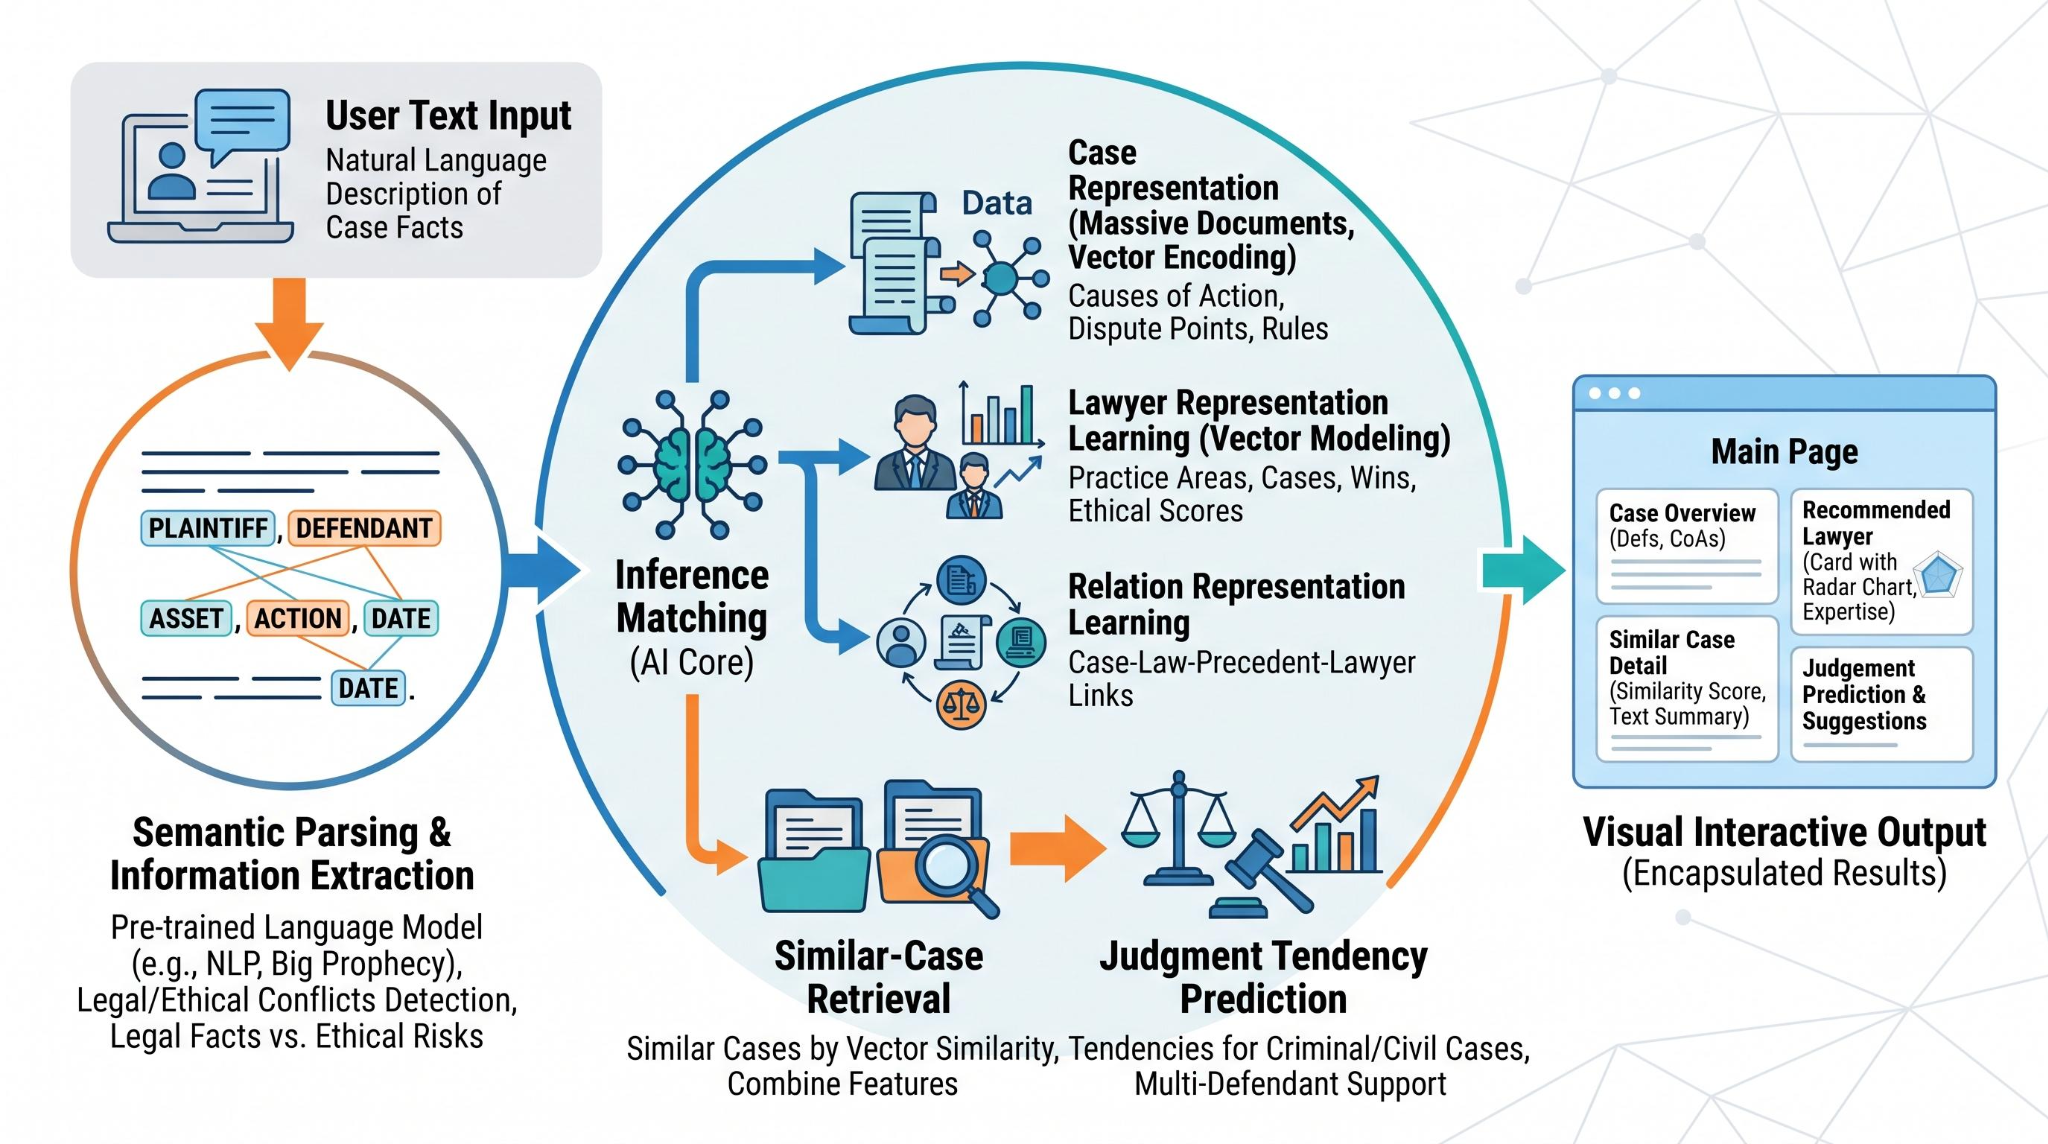
\includegraphics[width=1.0\linewidth]{figure/PicDoc_2026-10-30+21_09_27.png}
\caption{Framework of Legal Ethics Assistant.}
\label{fig:framework}
\end{figure}

\begin{figure}%[tbhp]
\centering
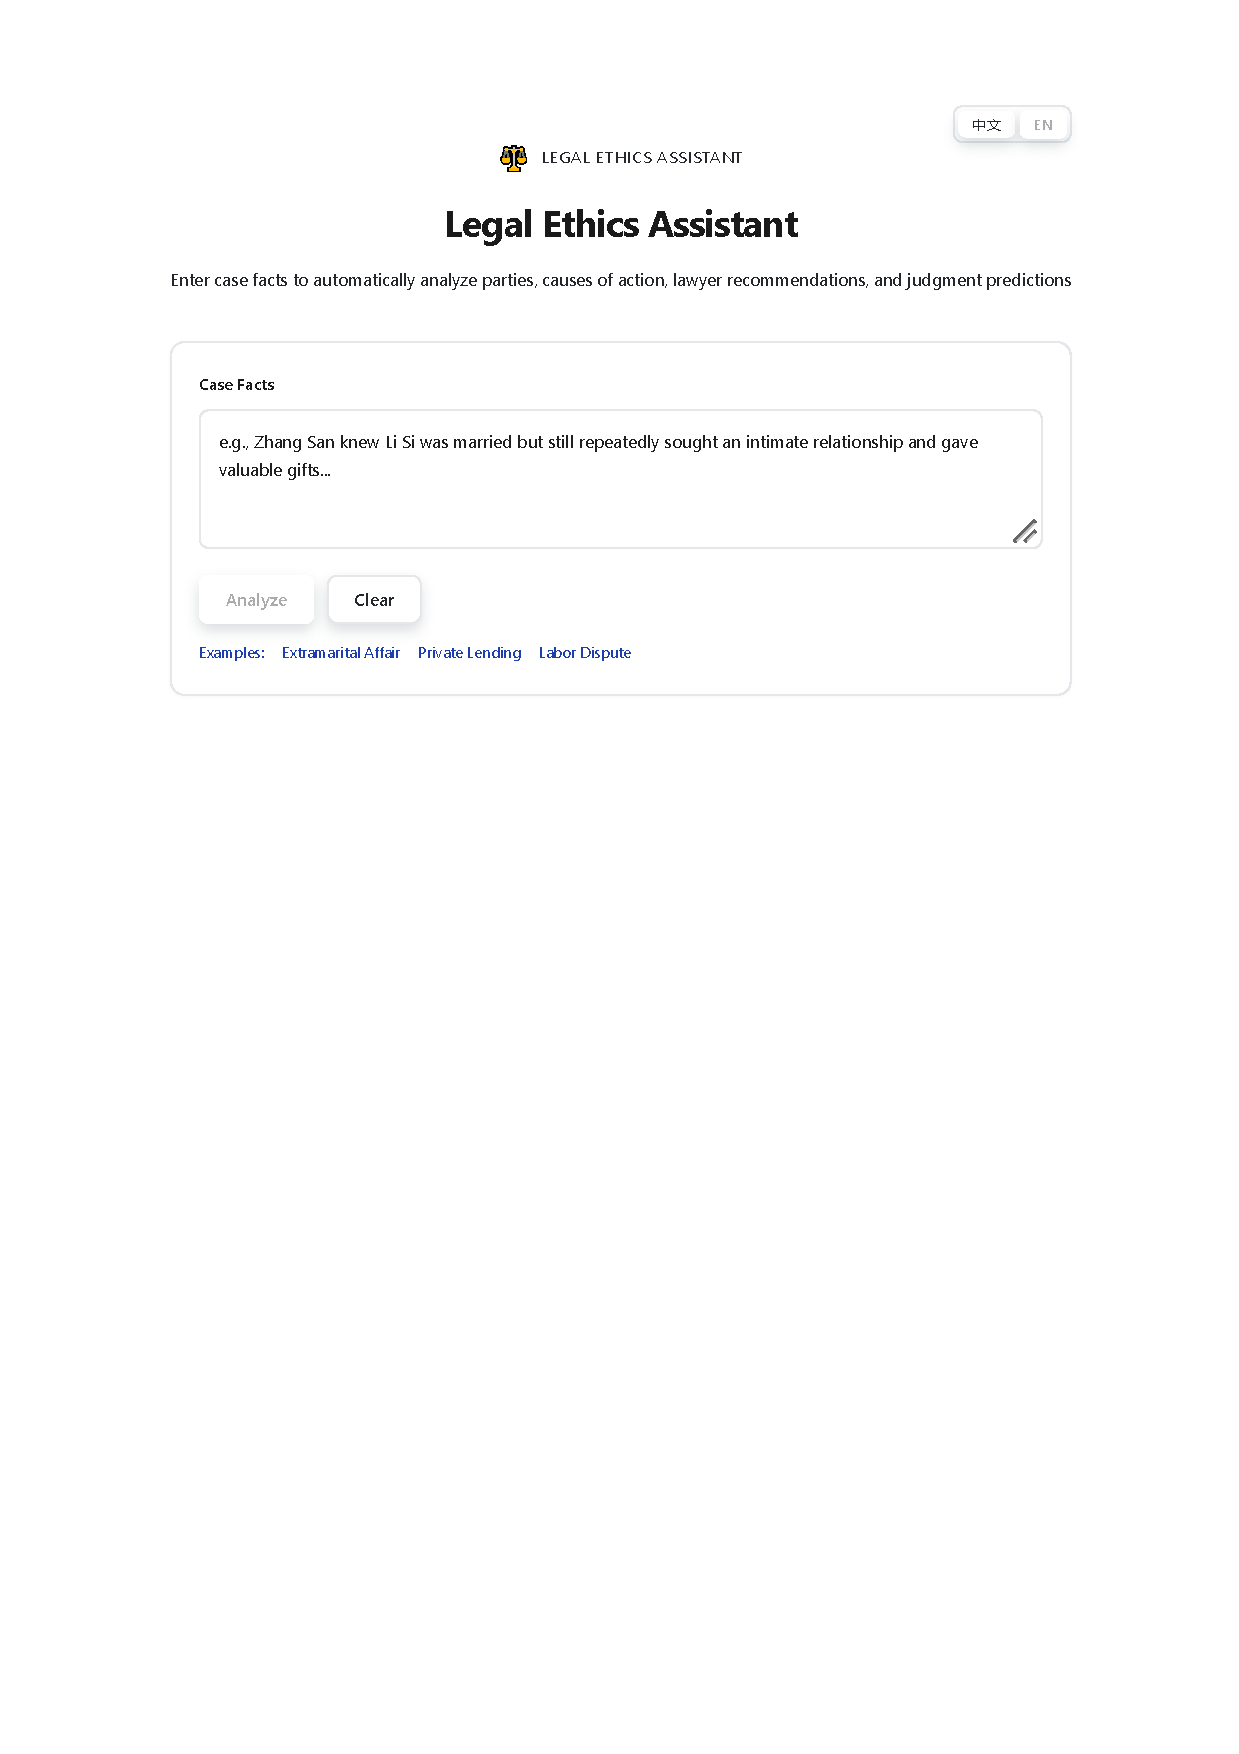
\includegraphics[width=1.0\linewidth]{figure/index.pdf}
\caption{Case fact input page of Legal Ethics Assistant.}
\label{fig:index}
\end{figure}

\begin{figure}%[tbhp]
\centering
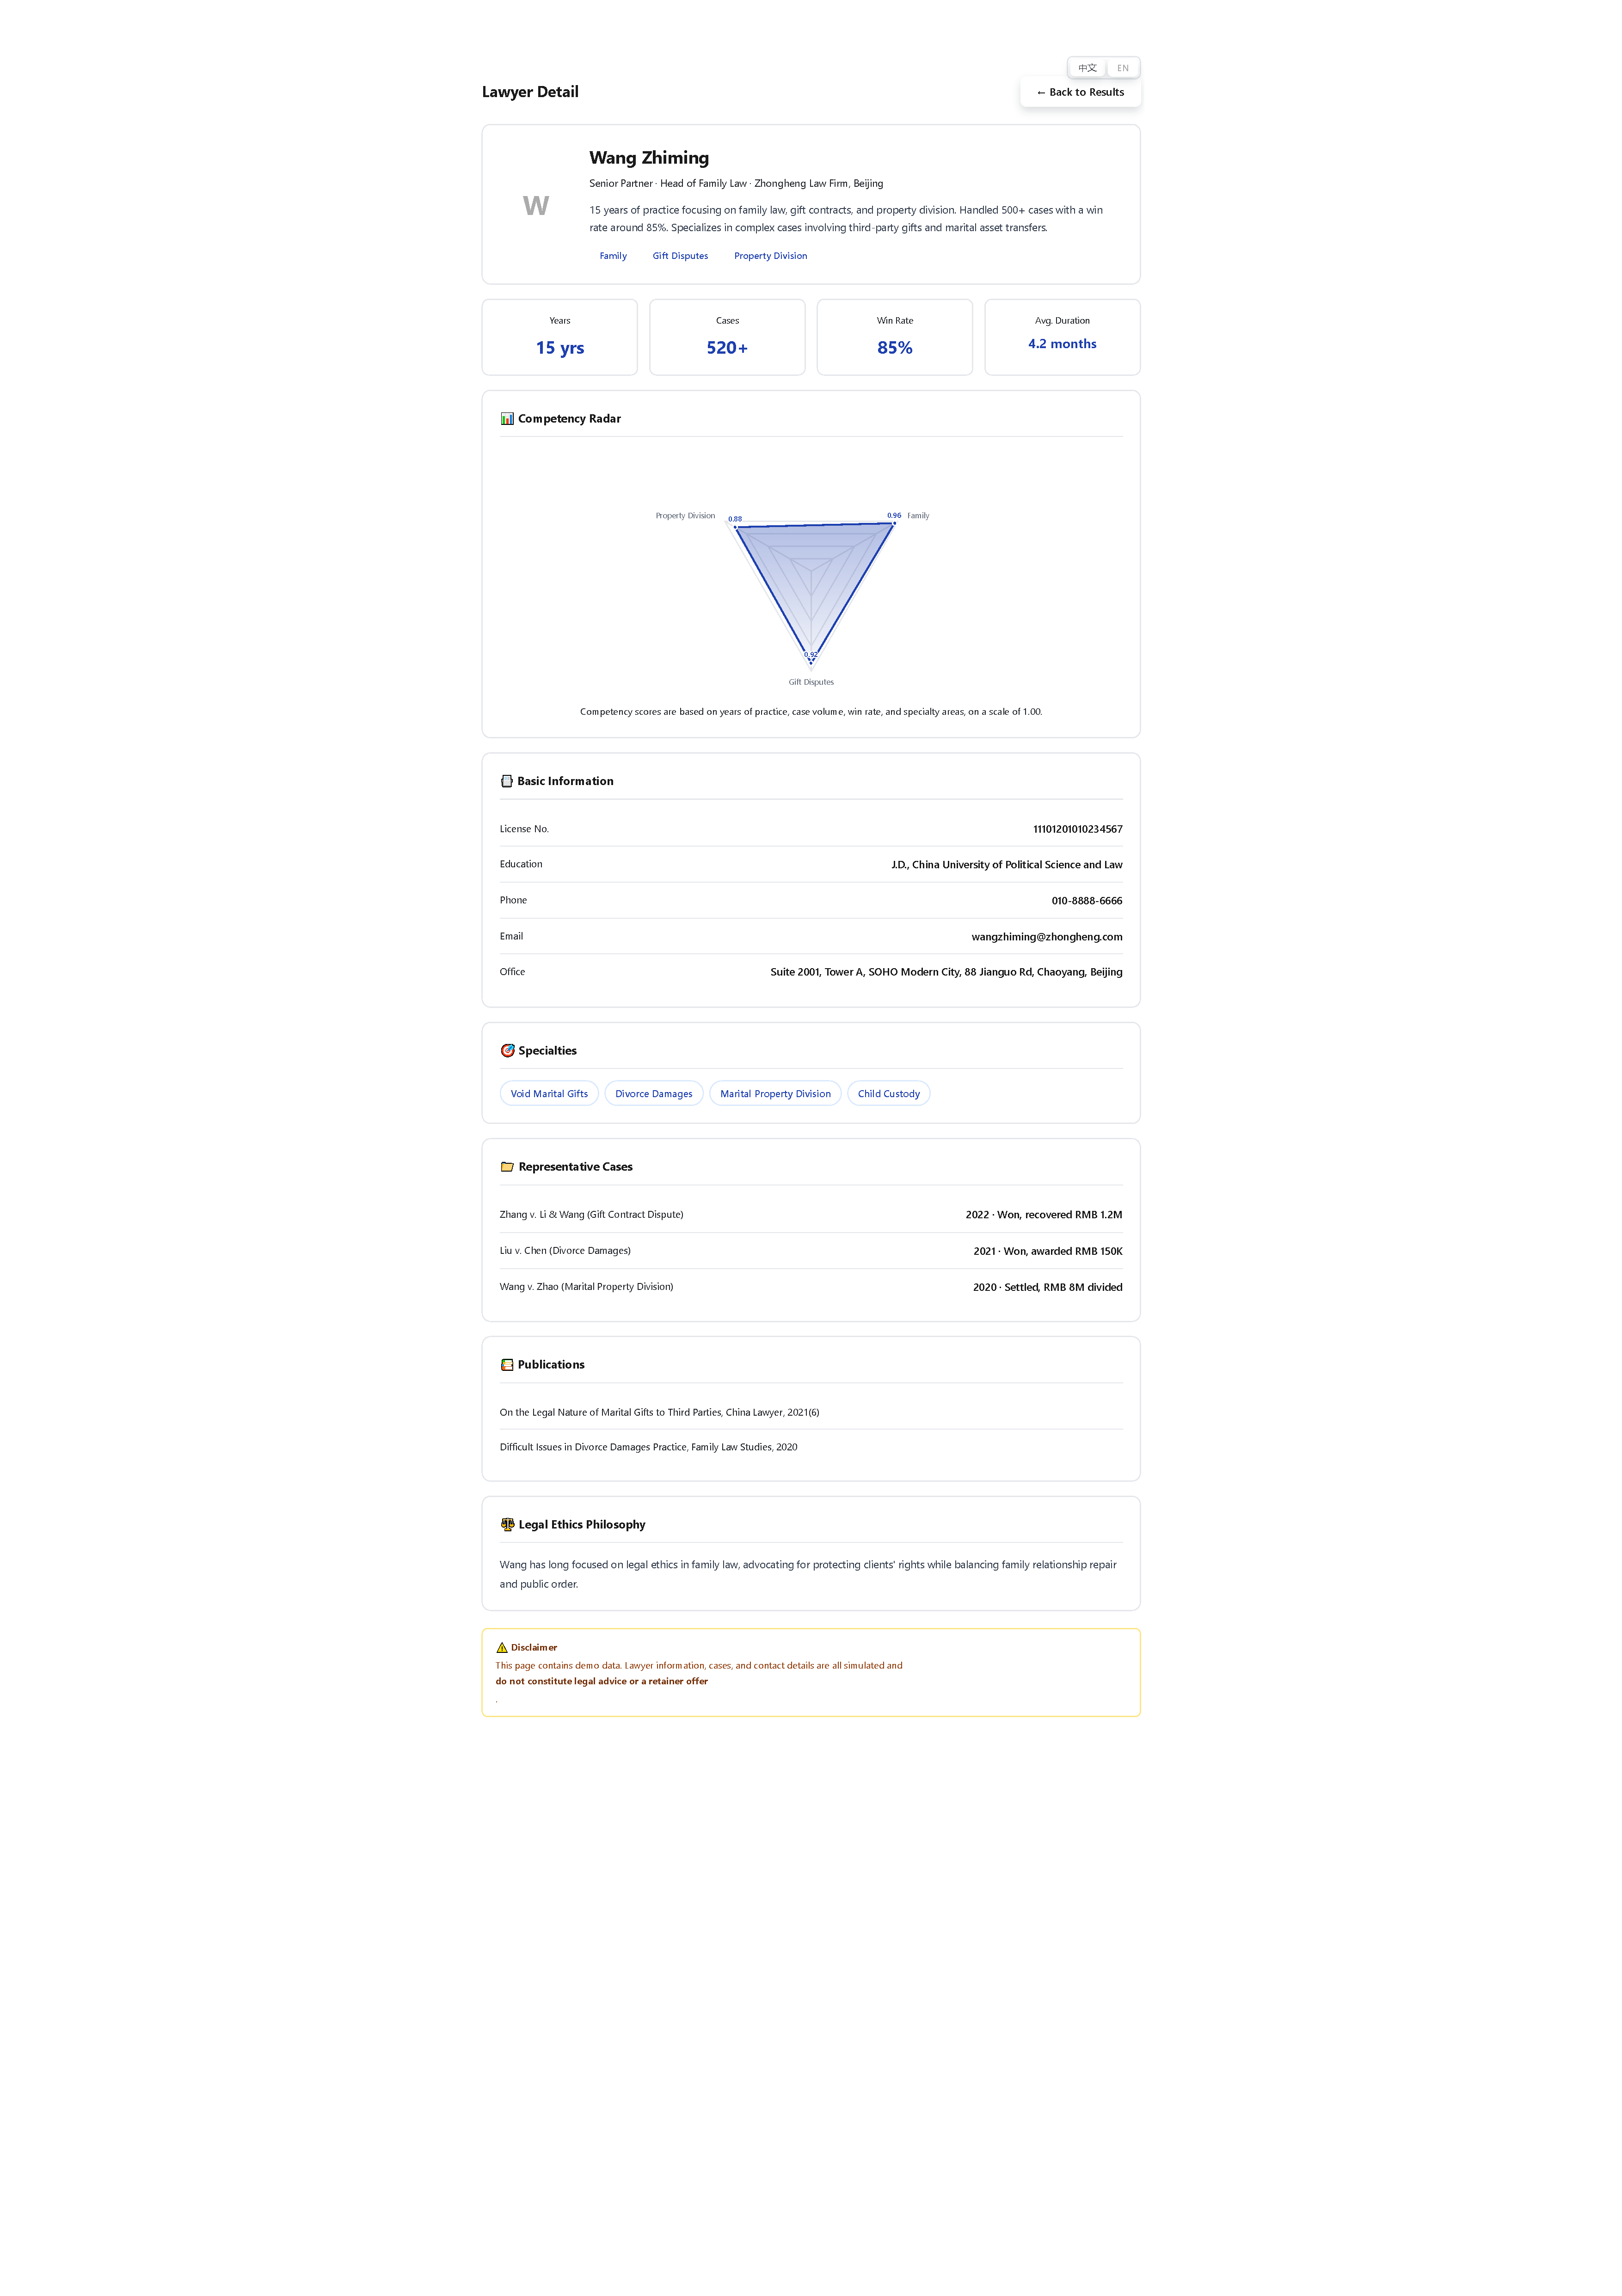
\includegraphics[width=0.8\linewidth]{figure/lawyer.pdf}
\caption{Lawyer detail page of Legal Ethics Assistant.}
\label{fig:lawyer}
\end{figure}

% \begin{figure}%[tbhp]
% \centering
% 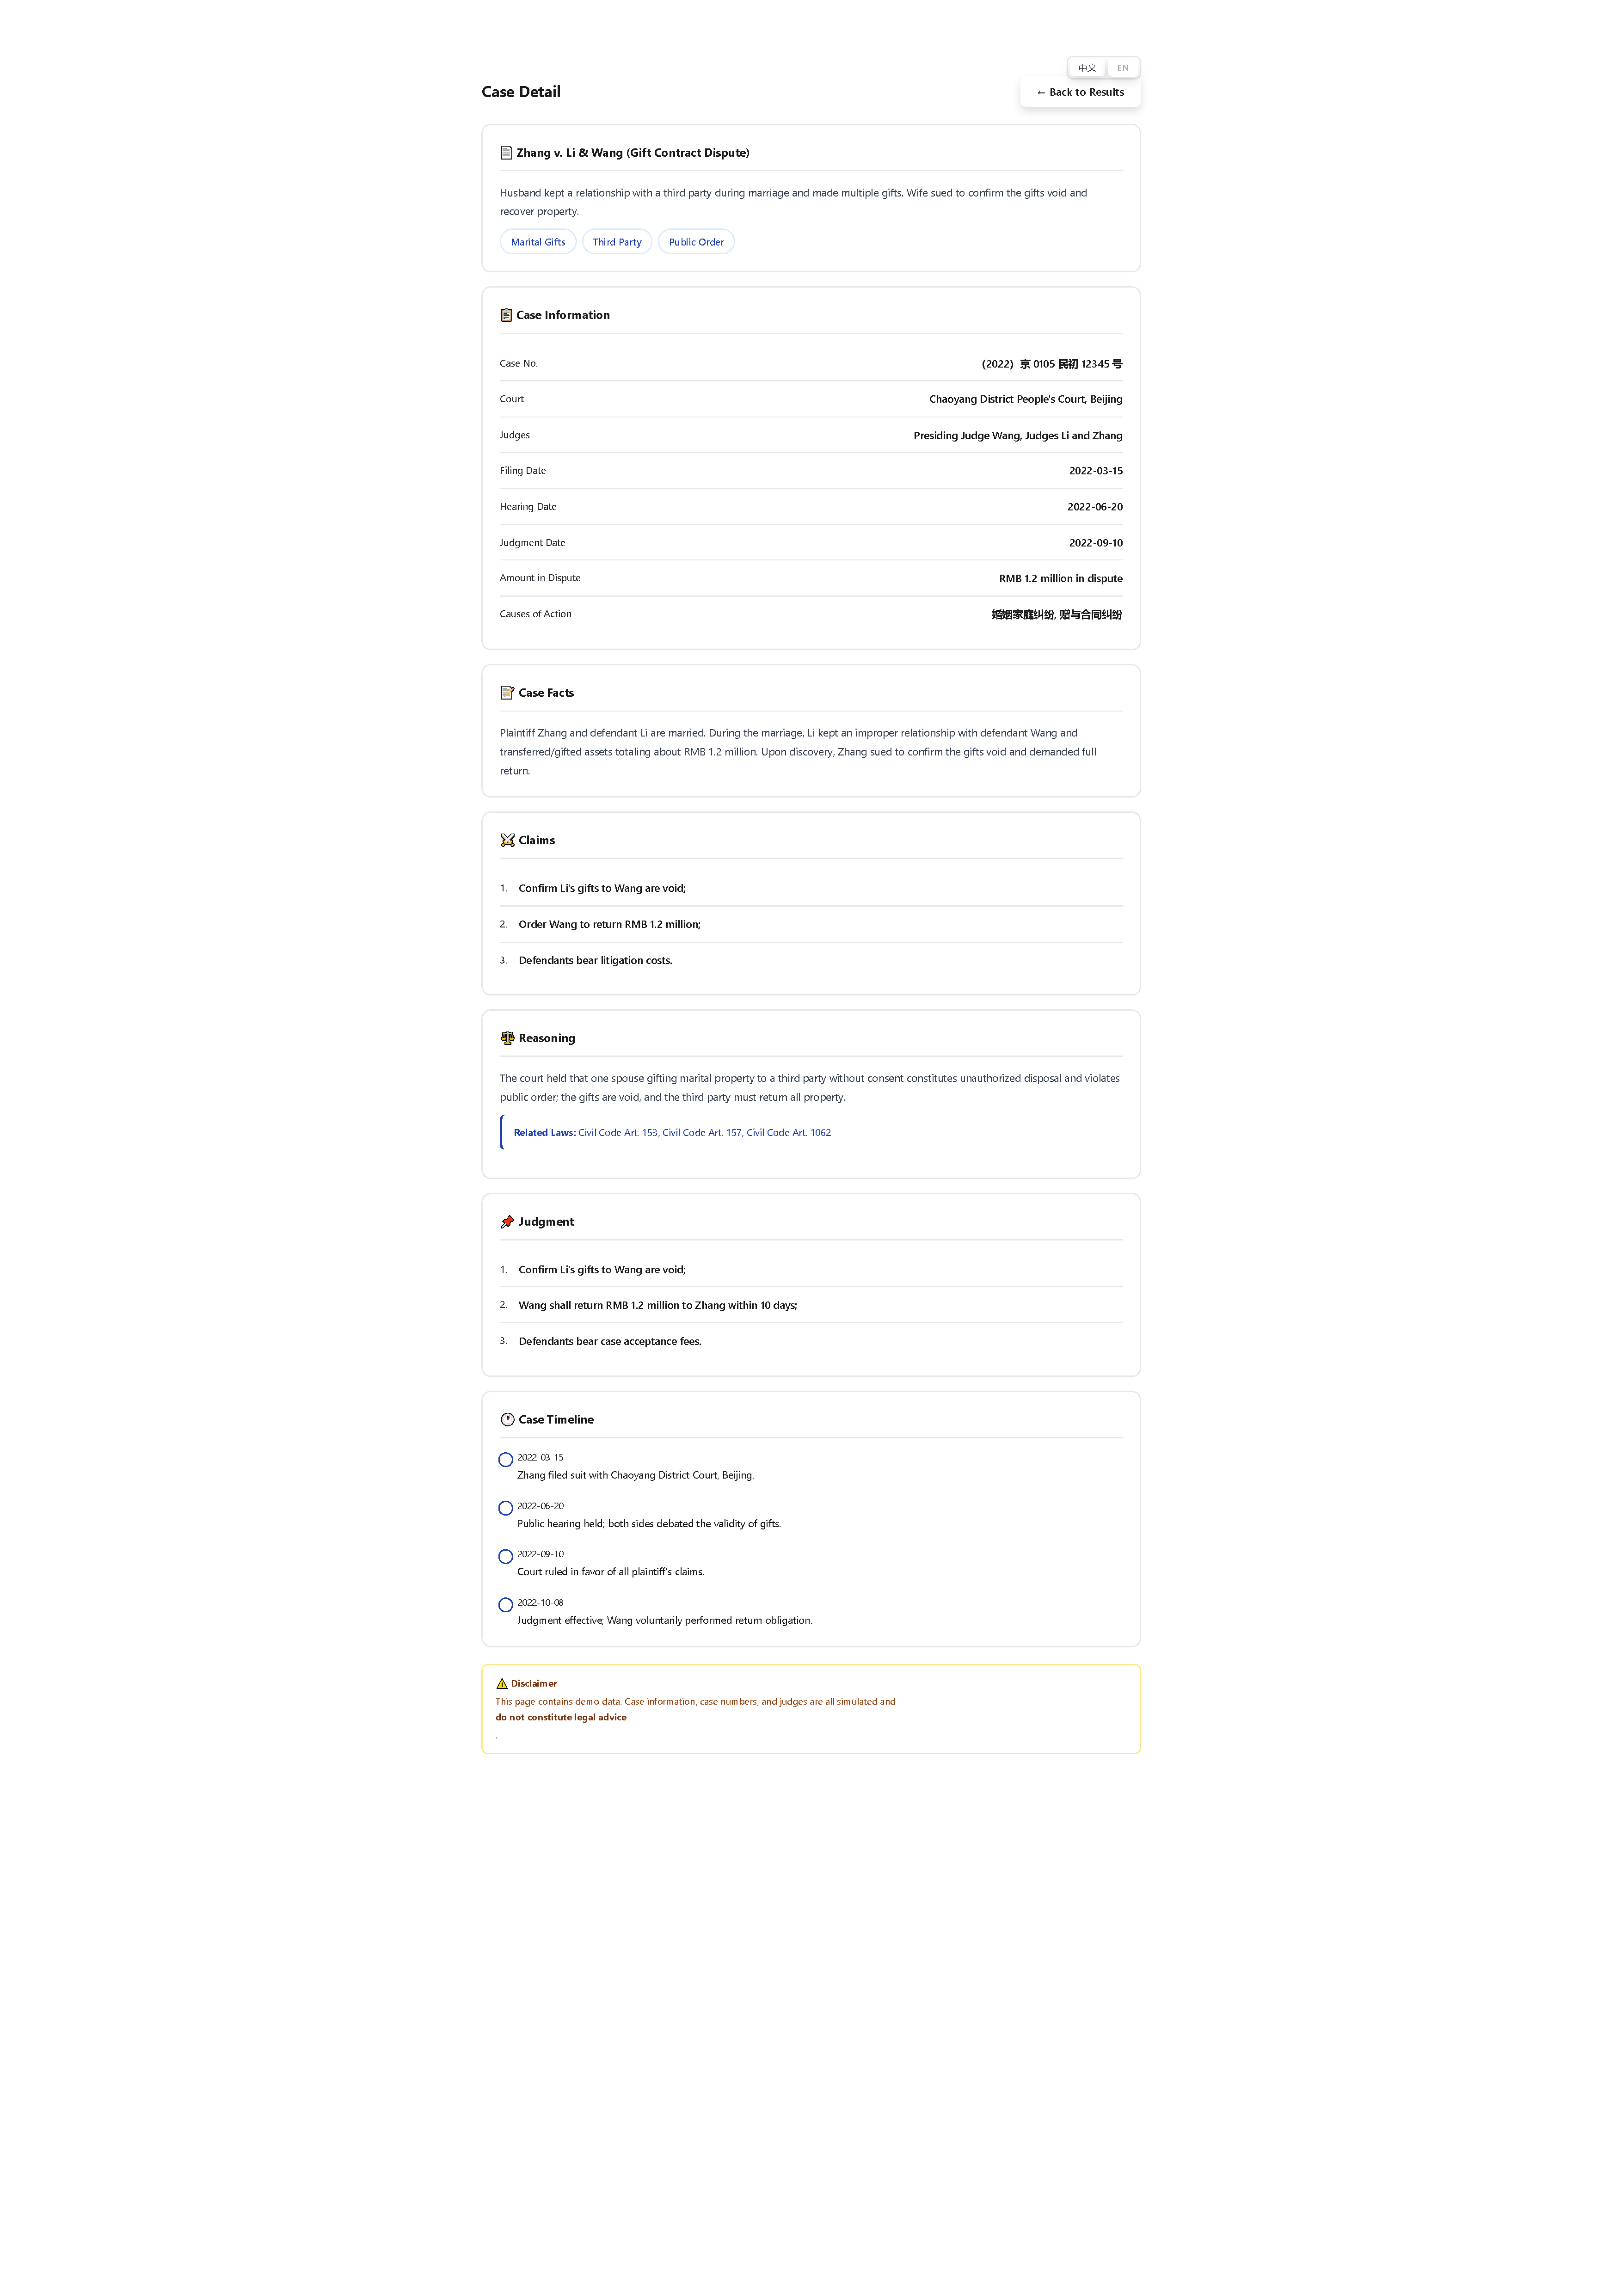
\includegraphics[width=.7\linewidth]{figure/case.pdf}
% \caption{Case detail page of Legal Ethics Assistant.}
% \label{fig:case}
% \end{figure}

\begin{figure}%[tbhp]
\centering
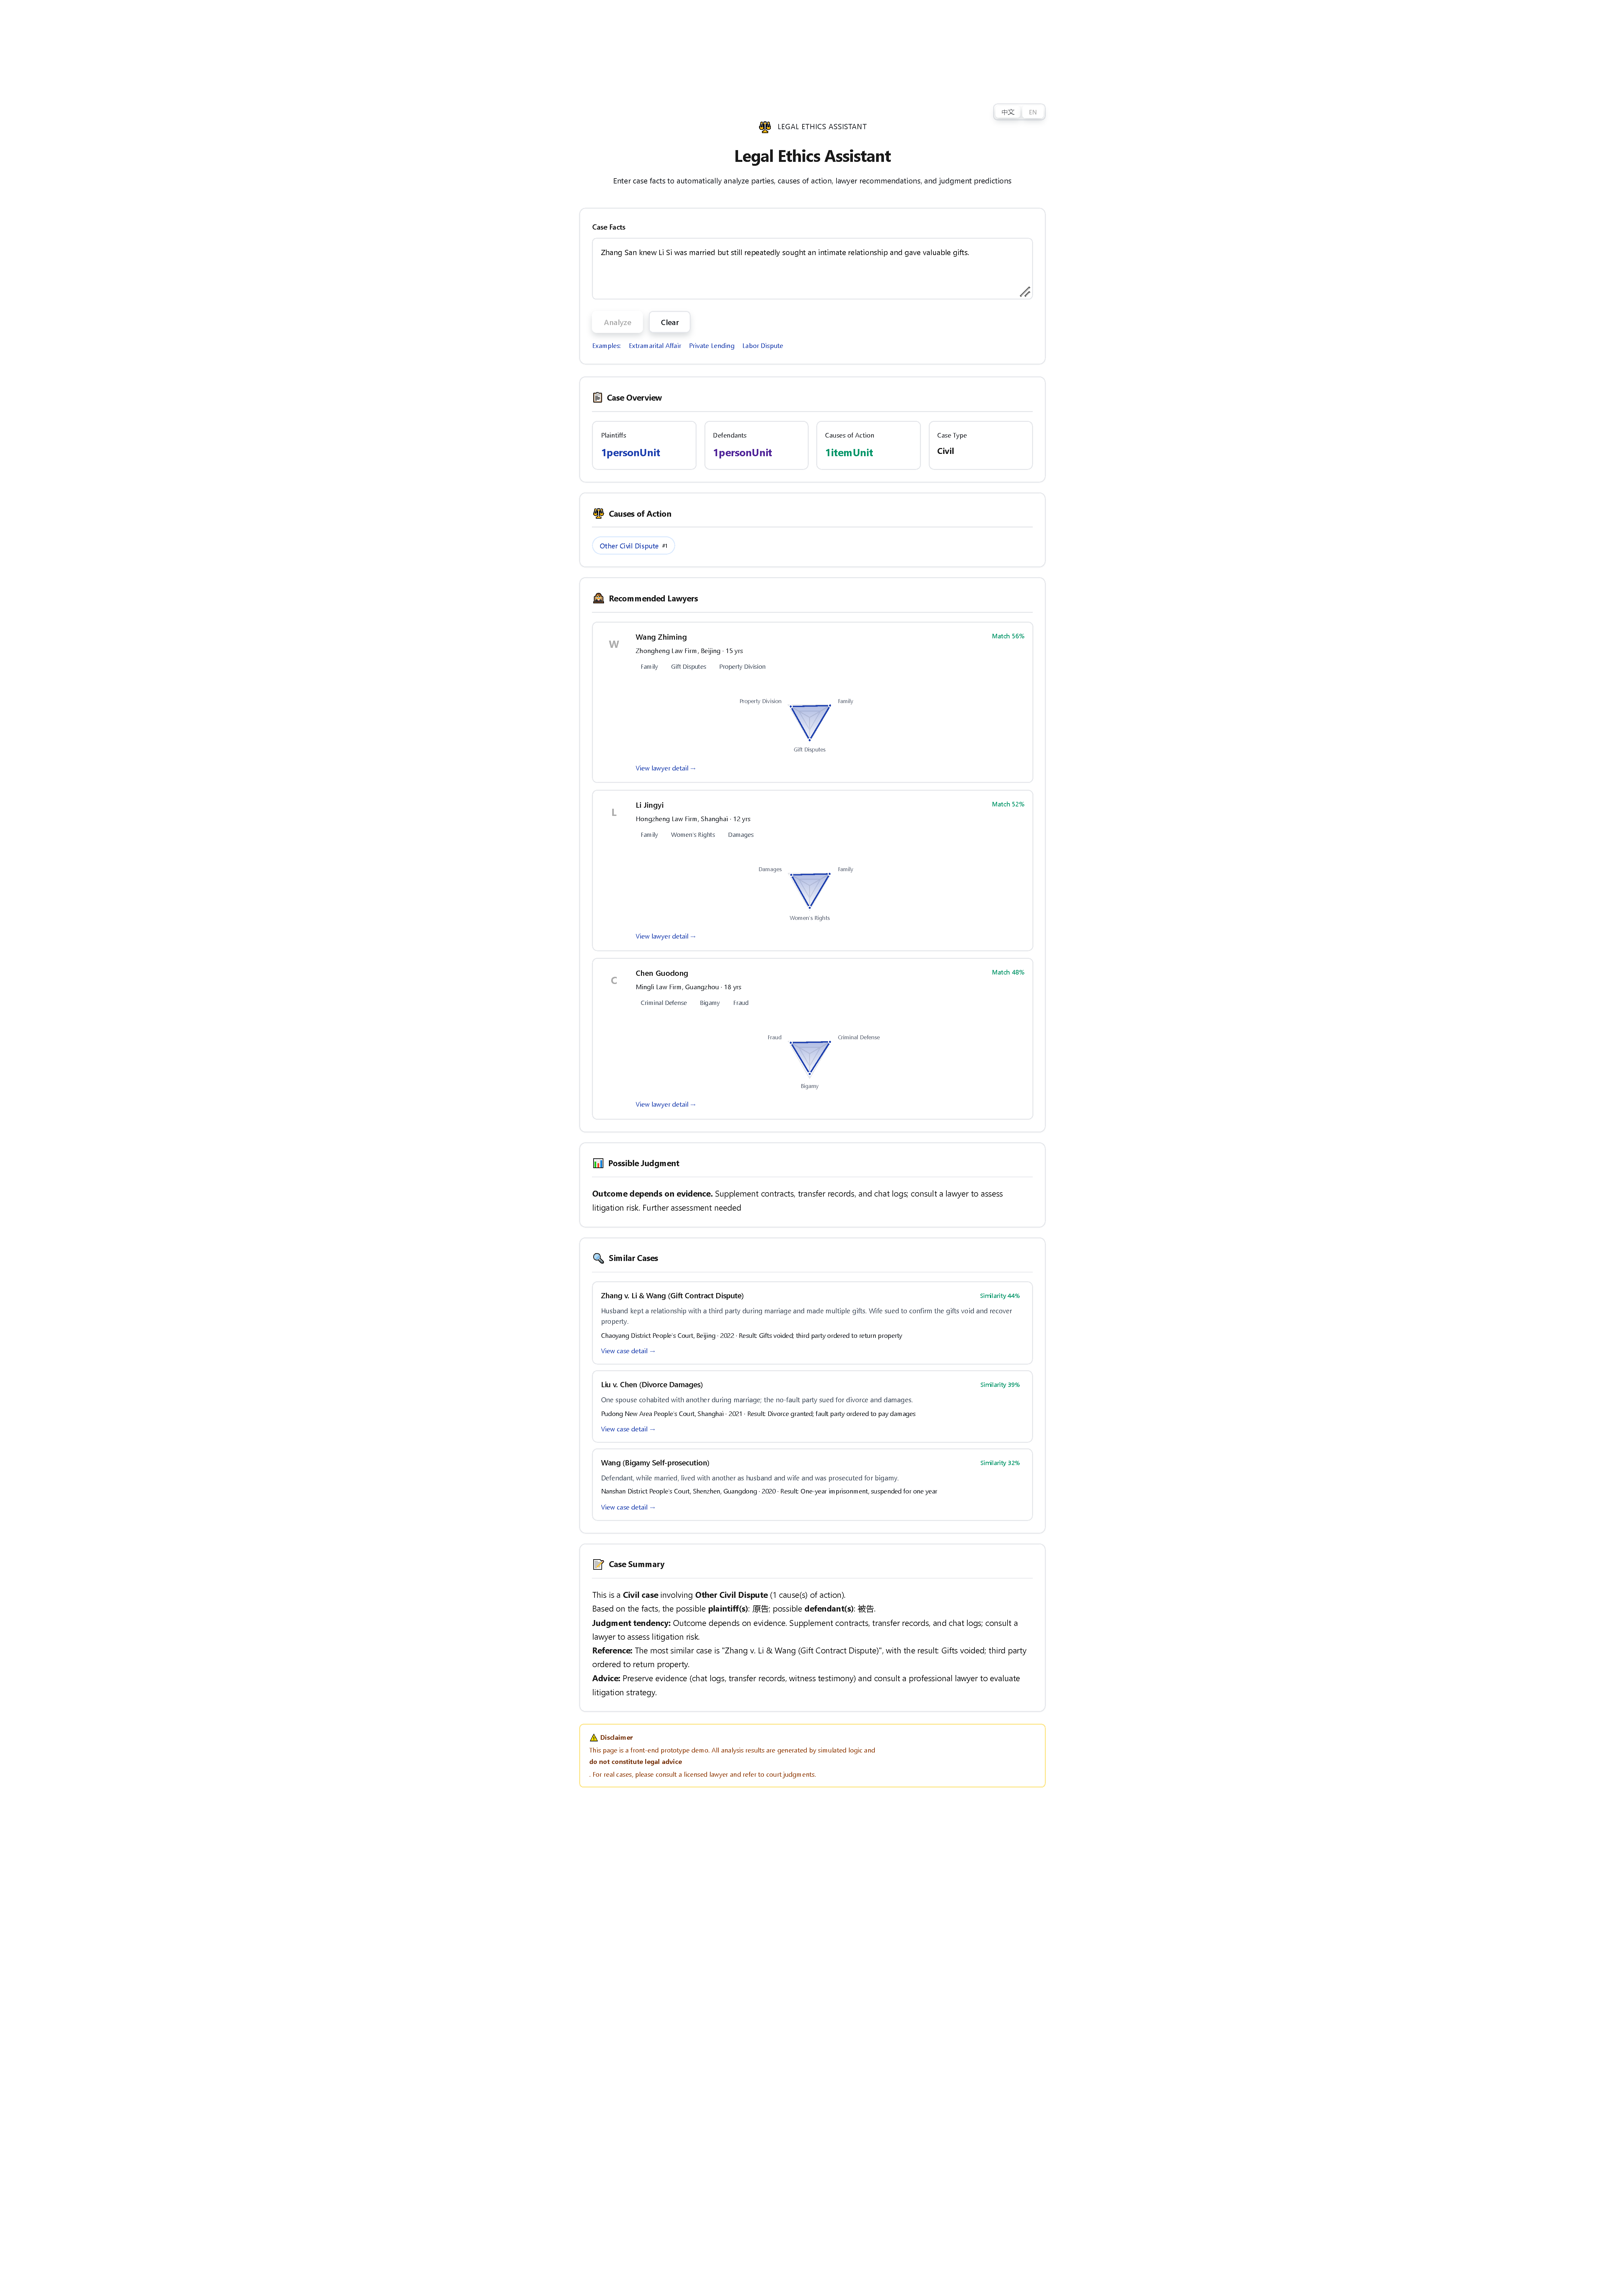
\includegraphics[width=.7\linewidth]{figure/mainpage.pdf}
\caption{Main page of Legal Ethics Assistant.}
\label{fig:mainpage}
\end{figure}

\section{Conclusion}

This paper proposes a Legal Ethics Assistant tool for both non-professional users and legal professionals. This tool utilizes a large amount of publicly available court judgment data online, recommending lawyers and similar cases based on case descriptions, and providing judgment tendencies and suggestions. This helps mitigate risks before or in the early stages of legal proceedings, bridging the information gap for those involved or legal professionals. By integrating lawyer and case information and continuously supplementing data and knowledge, the reliability and effectiveness of the recommendations are improved. Finally, by providing judgment tendencies and suggestions, the assistant guides users, realizing the positive impact of technology on society and maintaining long-term social stability.

The system is of significant novelty and research importance.
At the practical level, the system reduces the cost of initial legal consultation for the public, helps parties identify case risks in advance, rationally anticipate judgments, and reduce irrational rights protection; it also assists grassroots legal service personnel in improving work efficiency.
At the technical level, this solution provides an implementation approach for explainable legal AI that integrates ethical constraints, knowledge graphs, and dual-representation learning, balancing AI's deductive capabilities with the rigor required by legal scenarios.
At the value level, the project adheres to a "Tech for good" orientation, clearly defining the boundaries of AI-assisted tools, ensuring it does not replace practicing lawyers, and balancing the needs of inclusive legal services with legal security risks, providing valuable reference for AI-enabled grassroots social governance.

% 法律智能旨在为人们提供法律帮助。法律从业者以及当事人等法律用户由于专业性和平常接触不到的原因，很少被研究。大量公开的裁判文书数据和律师接案记录让我们可以了解他们的从业情况并进行科学研究。法律领域的研究主要集中在心理层面或道德层面，例如对各文明法律发展的研究，以及某一社会现象可能涉及的法律研究。更偏向理工理论类的研究有犯罪心理学，博弈论囚徒困境等。随着人工智能与大数据技术的发展，数据处理与分析技术开始应用于法律领域，近年来，学者开始对法律文书展开研究，常用的方法是用自然语言处理技术分析法律文书。由于其领域特性，法律文书可以被组成为半结构化数据，一般分为人员与组织信息、案件事实描述、持有证据和判决结果。由于判决结果种类有限，一般可以作为分类任务进行预测，例如刑事法律判决预测一般预测相关发条、判决罪名、刑期，民事一般预测原告的诉求是否被支持，例如支持、部分支持和不支持。此外，还有庭审观点生成、类案检索、法律问答等研究都是通过法律文本，也有基于民事判决预测的OOD捷径学习的研究。其中研究最广也最久的是刑事法律判决预测。最早是通过支持向量机对法条进行预测，而后扩展到罪名和刑期。在以BERT、GPT为代表的预训练模型飞速发展的时期，法律智能同时也取得了飞速发展。由此衍生出可解释法律判决预测和多被告法律判决预测等。
%     类案检索是指在案件数据库中检索相似案件的技术。定义相似案件的方法有很多种，例如案件类型相似、法律元素相似等。清华大学刘逸群老师组对此展开了深入研究。刘逸群老师在检索、搜索引擎领域有一定的技术积累，将相关方法迁移到类案检索领域，并借助传统BM25和BERT预训练方法构造了LeCaRD数据集，在此基础上展开研究。基于预训练模型和大语言模型的类案检索方法可以分为三类，第一类是基于预训练模型训练方法的研究，一般是对BERT模型的改进与扩展。第二类是基于用户行为的案件检索方法。这一类方法融合了用户行为，例如在相似案件标注时的点击或页面停留时间反映了案件的相关程度，包括使用用户查询对话记录的对话式类案检索方法。第三类是基于智能体的对话式类案检索方法，因为涉及智能体的方法需要产生交互，一般通过对话式的方法，借助人类标注流程，检索相似的案件。其中包括基于大语言模型的方法。现有基于大语言模型的方法主要是通过提示词抽取信息，生成相关知识融合案件文本对案件进行表征，最后通过相似度算法查找最相关案件。

    

% 类案检索是法律智能中的一项基本任务。现有的评估类案检索方法指标主要是precision和ndcg.然而，还没有使用下游任务评价类案检索方法。

% ~\footnote{Our code are available at \url{https://github.com/BounceDude/XXX}}

% 随着互联网的发展与法院案件的逐渐增多，类案检索的需求越来越迫切。
%     在保证案件判决质量的同时，也要遵循"同案同判"的原则，相关地，最高人民法院发布指导性文件~\footnote{\url{https://www.chinacourt.org/law/detail/2020/07/id/150187.shtml}}。
%     目前市面上有法律案件检索网站，包括把手案例~\footnote{\url{https://www.lawsdata.com/}}、北大法宝~\footnote{\url{https://www.pkulaw.com/}}等，但对于类案检索任务仍然有很大的研究空间。

%     场景

%     现有的基于类案检索的研究

%     事实上，在解决类案检索任务时，有很多技术和领域上的挑战。
%     包括如何定义案件的相似，以及如何根据法律领域的特点检索相似案件。

%     为此，我们提出了一种类案检索方法。

%     % 贡献：
%     % 我们提出了一种通过律师推荐验证类案检索模型的方法。

%     \section{Related Works}
%     \subsection{Text Matching}

%     文本匹配任务被广泛研究，包括在教育、职场、法律领域。
%     文本匹配方法包括传统的TF-IDF、BM25，近年来的预训练模型和大模型。

%     类案检索任务相较于其它领域，具有更强的专业性，例如如何定义案件的相似。

% \subsection{Legal Case Retrieval}

%     在一般的网络搜索中，用户行为受到了广泛的关注兴趣和受益相关的IR任务[57–60]。具体地说,
% 领域专业知识和任务难度是两个影响因素。White等人[61]进行了纵向分析研究领域专业知识对网络
% 搜索行为的影响在四不同的领域(医学、金融、法律和计算机科学)。Mao等[62] 进一步进行了实验
% 研究领域专业知识在探索性搜索中的影响，涉及环境、医学和政治领域的任务。至于任务困难，多方
% 研究努力分析在网络搜索中对搜索行为的影响，并建立相应的预测模型[63–65]。我们注意到，对于
% 任务难度的定义没有共识。一些研究[66,67] 将难度定义为用户对任务复杂性的主观感知，而一些研
% 究[63, 68] 考虑了客观测量，如正确性、任务性能。专业搜索被定义为支持或解决不同领域(如专利、
% 法律、医疗等)专业人员工作任务的活动[69,70]。
% 因此，除了建立语义案例匹配模型外，近年来的一些工作也将重点放在案例检索中的用户系统交
% 互方面。Shao 等人[71] 进行了一项用户研究，调查了法律案件检索中的用户行为，并说明了与网络搜
% 索场景的显著差异，例如探索性。考虑到法律案件检索任务的复杂性，Liu等人[72]通过对用户的研
% 究，尝试将对话式检索模式应用到法律案件检索中，以帮助用户更好地表达自己的信息需求。值得注意
% 的是，这些研究中的任务仍然是基于客观法律知识的分类来设计的，如法律规则[2]或法律问题[72]。
% 此外，还有研究探索了对话式类案检索，包括在对话问题生成[73]、对话智能体[74, 75] 和与传
% 统类案检索的比较[72] 等方面的研究。Liu 等人开展了用户相关的类案检索研究，包括对用户决策过
% 程[76]、用户子主题标注[77]、用户意图分类[78]、用户决策相关性[79] 和用户行为[71] 的分析预测。
% 6
% 综上所述，现有的法律智能研究，如应用场景、模型开发、交互设计等方面，对政法领域用户有
% 待进一步进行系统的研究。针对律师、司法鉴定人员、公证员、调解员等法律服务执业人员，社区矫
% 正对象、戒毒对象、监狱服刑对象等特殊人群，以及庭审过程中的原告、被告、法官等政法领域用户
% 角色，我们展开对政法领域用户的用户表示研究，通过用户行为数据分析与挖掘，洞察用户偏好，了
% 解用户行为意图与需求，提高用户满意度。

% \section{PRELIMINARIES}
% \subsection{Problem Formulation}

% Legal case retrieval task refers to finding cases relevant to a given
% query case from the candidate case set. Formally, given a query
% case q, and a set of candidate cases D, the task is to retrieve top-k
% relevant cases $D_q=d_1^*,d_2^*,\cdots ,d_k^*$ from a large candidate pool.



% \section{ArticleLCR}


% \subsection{overview}
% In this section, we describe our structure-aware pre-trained lan-guage
% model for legal case retrieval in detail.
% In order to integrate the structural knowledge into the language
% model, we simulate the writing process of legal case documents and
% propose the SAILER, which is shown in Figure 3. SAILER mainly
% consists of three components, i.e., Fact Encoder, Reasoning Decoder,
% and Decision Decoder. Speciffcally, in the pretraining process, aBERT-like encoder is used to generate a vector representation ofthe Fact, and two shallow decoders are used to reconstruct the textof the Reasoning and Decision sections. Detailed descriptions aboutthe SAILER are as follows.
% \subsection{Fact Encoder}

% In the Fact Encoder, we first randomly replace some tokens of the Fact with a special token [MASK]. Only a small percentage of tokens is replaced, as the majority of the Fact need to be preserved.

% In particular, We define the facts as $F=\left[f_1, f_2, \ldots, f_n\right]$ and the masked token set as $m(F)$, where $f$ denotes tokens and $n$ denotes the length of Fact. So the rest tokens can be represented as $F \backslash m(F)$. Then, the masked input $F_{\text {mask }}$ is transformed into a sentence vector by the Fact Encoder $\phi_F(\cdot)$. Following the previous work [9, 14], the final hidden state of the [CLS] token is taken as the representation of the entire sentence:


% \begin{equation*}
% h_F=\phi_F\left(F_{m a s k}\right) \tag{2}
% \end{equation*}



% Similar to Bert, We input the masked facts into the encoder to recover $m(F)$ and compute mask language modeling (MLM) loss as one of our pre-training objectives. Specifically, the MLM loss $L_{M L M}$ is defined as:


% \begin{equation*}
% L_{M L M}=-\sum_{x^{\prime} \in m(F)} \log p\left(x^{\prime} \mid F \backslash m(F)\right) \tag{3}
% \end{equation*}




% \subsection{Reasoning Decoder}

% As mentioned above, the Reasoning section contains all the key legal elements of the case. Therefore, we design the Reasoning Decoder to model the logical relationships between Reasoning and Fact, aiming to improve the alignment between the focus of the encoder and the underlining key legal elements in case documents.

% Specifically, we construct the Reasoning Decoder through polluting the original text of the Reasoning section $R=\left[r_1, r_2, \ldots, r_n\right]$. We split the Reasoning text into tokens and randomly select a subset $m(R)$ for masking. An aggressive mask ratio $(30 \%-60 \%)$ is adopted for language reconstruction. In addition, the dense vector $h_F$ replaces the original [CLS] vector which is commonly used as the beginning of decoder inputs. The whole decoder input is formalized as:


% \begin{equation*}
% \left[h_F, e_{r_1}+p_{r_1}, \ldots, e_{r_n}+p_{r_n}\right] ; \tag{4}
% \end{equation*}


% where $e_{r_k}$ and $p_{r_k}$ denote the embeddings and extra position embedding of $r_k$. In this way, the learning objective of the Reasoning Decoder is formulated as:


% \begin{equation*}
% L_{R E A}=-\sum_{x^{\prime} \in m(R)} \log p\left(x^{\prime} \mid\left[h_F, R \backslash m(R)\right]\right) \tag{5}
% \end{equation*}


% The Reasoning Decoder needs to rely on $h_F$ to recover the masked Reasoning section, which forces the $h_F$ to focus on useful information related to the Reasoning section in the facts. By this design, SAILER enhances attention to the key legal elements and captures the long dependencies between Facts and Reasoning.

% \subsection{Decision Decoder}

% Legal Judgment Prediction (LJP) aims to predict the judgment results of a case based on the fact description [11]. If two cases have the same charges and law articles, then their dense vectors should be closer in the vector space. In this part, the Legal Judgment Prediction is modeled as a text-to-text task by using Decision Decoder, which helps the vectors have a stronger discriminatory ability.

% For Chinese legal cases, the Decision usually consists of the relevant law articles, charges, and terms of penalty. Given a Decision section $D=\left[d_1, d_2, \ldots, d_n\right]$, we mask it according to its specified
% format. Concretely, the Decision is usually formatted as follows: According to the Criminal Law of the People's Republic of China $\left[z_1\right]$, the defendant committed $\left[z_2\right]$ and was sentenced to $\left[z_3\right]$, where $z_1$ denotes the specific law articles, $z_2$ represents the charges, and $z_3$ is the term of penalty. We use $\mathcal{Z}$ to denote all masked tokens.

% In some countries where the Decision does not have a specific format, we select a certain percentage of words with high TF-IDF [1] values to mask. For convenience, we still name the masked tokens as $\mathcal{Z}$.

% The Decision Decoder also relies on the dense vector $h_F$ to recover the original decision. Specifically, the input of the Decision Decoder is:


% \begin{equation*}
% \left[h_F, e_{d_1}+p_{d_1}, \ldots, e_{d_n}+p_{d_n}\right] ; \tag{6}
% \end{equation*}


% where $e_{d_k}$ and $p_{d_k}$ denote the embeddings and extra position embedding of $d_k$. The Decision Decoder is trained with the objective:


% \begin{equation*}
% \left.L_{D E C}=-\sum_{x^{\prime} \in \mathcal{Z}} \log p\left(x^{\prime} \mid\left[h_F, D \backslash \mathcal{Z}\right)\right]\right) \tag{7}
% \end{equation*}



% In short, Decision Decoder cleverly models the Legal Judgment Prediction task to help generate discriminative vectors.


% \subsection{Article Decoder}

% We define the facts as $F=\left[f_1, f_2, \ldots, f_n\right]$ and the masked token set as $m(F)$, where $f$ denotes tokens and $n$ denotes the length of Fact.

% \begin{equation*}
% h_F=\phi_F\left(F_{m a s k}\right) \tag{2}
% \end{equation*}

% \begin{equation*}
% \left.L_{ART}=-\sum_{x^{\prime} \in \mathcal{Z}} \log p\left(x^{\prime} \mid\left[h_F, D \backslash \mathcal{Z}\right)\right]\right) \tag{7}
% \end{equation*}

% \subsection{Learning}

% During pre-training, we aim at optimizing the following training objectives:


% \begin{equation*}
% L_{\text {Total }}=L_{M L M}+L_{R E A}+L_{D E C}+L_{ART} \tag{8}
% \end{equation*}


% After pre-training, we drop both decoders and fine-tune the encoder. The purpose of fine-tuning is to make the query closer to related cases in the vector space compared to the irrelevant ones. Thus, given a query case $q$, let $d^{+}$and $d^{-}$be relevant and negative cases, the loss function $L$ is formulated as follows:


% \begin{equation*}
% L\left(q, d^{+}, d_1^{-}, \ldots, d_n^{-}\right)=-\log \frac{\exp \left(s\left(q, d^{+}\right)\right)}{\exp \left(s\left(q, d^{+}\right)\right)+\sum_{j=1}^n \exp \left(s\left(q, d_j^{-}\right)\right)} \tag{9}
% \end{equation*}


% Following previous work [26, 41], the negative samples $d^{-}$are BM25 hard negatives. During training, it is computationally expensive to sample many negative samples for each query case. Therefore, in-batch negatives [16] are adopted for contrastive learning which to take full advantage of negative samples in the same batch. Specifically, if there are $B$ queries in a batch, each with one positive and $N$ negative examples, then we can obtain at most $(B-1) *(N+1)$ in-batch negative examples for each query during training.


% \section{Experiments}
% \subsection{Datasets and Metrics}
% \subsection{Baselines}

%     SAILER：一个法律领域的文本编码器。

%     \subsection{Implementation Details}

% \subsection{Overall Performance}

% \subsection{Ablation Study}

% \subsection{Hyperparameter Analysis}

% \subsection{Case Study}
% \subsection{Visual Analysis}

% \subsection{律师推荐通过类案检索}

%     我们的目标是通过类案检索任务推荐律师，具体来说，就是搜索相似的案件，相似案件中出现的律师作为被推荐的律师。

%     我们通过律师推荐任务来验证我们提出的类案检索方法。
%     也就是说，通过类案检索方法检索相似的案件，案件中出现的胜诉的律师作为本案件的推荐律师。
%     推荐的律师通过LawyerPAN模型~\cite{an2021lawyerpan}预测是否能够在这个案件中获得胜利。
%     由于LeCaRD~\cite{ma2021lecard}数据集中没有参与的律师，我们通过LeCaRD数据集训练类案检索模型，再在LCHR~\cite{an2021lawyerpan}数据集上进行验证。
%     此外，因为LawyerPAN模型包含参与案件的所有律师，而我们假设被验证的案件是发生但未经过诉讼，在诉讼之前推荐律师，所以我们只采用LawyerPAN模型的anticipatory module部分预测。

% \subsubsection{律师推荐在类案检索方法}

%     我们提出方法与Baseline的实验效果如表所示。
%     从实验结果可以看出，

% \subsubsection{律师推荐在提出的类案检索方法}

%     为了更进一步验证我们提出方法在律师推荐任务上的效果，我们设置了所有参与本案的律师、参与本案的胜诉的律师和各领域条件。
%     实验效果如表所示。


% \begin{table}
% % \setlength{\abovecaptionskip}{0pt}
% % \setlength{\belowcaptionskip}{0pt}
% % \renewcommand\thetable{2}
% \renewcommand\arraystretch{0.8}
% % \centering
% \caption{律师推荐在提出的类案检索方法的实验结果.}
% % \vspace{-0.3cm}
% \label{tab:Tab01}
% \begin{tabular}{ccc}
%     \toprule
%     \ \ \ \ \ \ 条件         & \ \ \ \ \ \ \ 胜诉率  & \ \ \ \ \ \       \\
%     \midrule
%     \ \  \# \ 所有参与本案的律师           & \ \ \ \ \ \ \ 0.4      & \ \ \ \ \ \ 29,015    \\
%     \ \  \# \ 参与本案的胜诉的律师             & \ \ \ \ \ \ \ 0.6     & \ \ \ \ \ \  772,920  \\
%     \ \  \# \  合同纠纷案件的所有参与本案的律师           & \ \ \ \ \ \ \ 0.4         & \ \ \ \ \ \  636      \\
%     \ \  \# \  合同纠纷案件的参与本案的胜诉的律师 & \ \ \ \ \ \ \ 0.5     & \ \ \ \ \ \ 1,020,090 \\
%     \bottomrule
% \end{tabular}
% % \vspace{-0.35cm}
% \end{table}

% \subsection{事实残缺与完整影响}

%     方法的输入部分采用事实描述，一般我们认为，输入事实是否完整会对相似案件的检索结果造成影响。
%     我们在一个案例中进行验证，分别输入案件事实的25%、50%、75%、100%，相似案件检索的结果如表 所示。


% \begin{table}
% % \setlength{\abovecaptionskip}{0pt}
% % \setlength{\belowcaptionskip}{0pt}
% % \renewcommand\thetable{2}
% \renewcommand\arraystretch{0.8}
% % \centering
% \caption{类案检索方法事实残缺与完整影响的实验结果.}
% % \vspace{-0.3cm}
% \label{tab:Tab01}
% \begin{tabular}{ccc}
%     \toprule
%     \ \ \ \ \ \ 输入比例         & \ \ \ \ \ \ \ NDCG@30  & \ \ \ \ \ \       \\
%     \midrule
%     \ \  \# \ 25\%           & \ \ \ \ \ \ \ 0.4      & \ \ \ \ \ \ 29,015    \\
%     \ \  \# \ 50\%             & \ \ \ \ \ \ \ 0.5     & \ \ \ \ \ \  772,920  \\
%     \ \  \# \  75\%           & \ \ \ \ \ \ \ 0.6         & \ \ \ \ \ \  636      \\
%     \ \  \# \  100\% & \ \ \ \ \ \ \ 0.7     & \ \ \ \ \ \ 1,020,090 \\
%     \bottomrule
% \end{tabular}
% % \vspace{-0.35cm}
% \end{table}


% \section{Conclusion}

\bibliographystyle{./IEEEtran}
\bibliography{./IEEEabrv,./IEEEexample}

% \vspace{12pt}
% \color{red}
% IEEE conference templates contain guidance text for composing and formatting conference papers. Please ensure that all template text is removed from your conference paper prior to submission to the conference. Failure to remove the template text from your paper may result in your paper not being published.

\end{document}
